%\thispagestyle{empty}
\section{Introduction}
\label{introductions}

The Compact Muon Solenoid (CMS)~\cite{JINST} is one of two general-purpose
detectors operating at the Large Hadron Collider (LHC) facility at CERN.
One of the central features of the CMS detector is a $6$-m diameter solenoidal
magnet operating at $3.8\,{\rm T}$, which enables the measurement of charged
particle momenta over more than four orders of magnitude, from less than
$100\MeVc$ to more than $1\TeVc$, by reconstructing their trajectories as they
traverse the CMS inner tracking system. The CMS Tracker, shown
in~Fig.~\ref{fig:tklayout}, consists of two main detectors: three
barrel layers and two endcap disks per side of silicon pixel detectors, covering
the region from $4\cm$ to $15\cm$ in radius, and within $49\cm$ on either
side of the collision point along the LHC beam axis; ten barrel layers and
twelve endcap disks per side of silicon strip detectors, covering the
region from $25$ to $110\cm$ in radius, and within $280\cm$ on either
side of the collision point along the LHC beam axis. The Tracker
acceptance extends up to a pseudo-rapidity of $\left | \eta \right | < 2.5$.


The precise and efficient determination of charged-particle momenta is a
critical component of the physics program of CMS, as it impacts the ability to
reconstruct leptons, charged hadrons, jets, and photon conversions, which
are the basic physics objects needed to understand $pp$ collisions at the LHC.
Standard reconstruction of tracks in
the CMS Tracker is seeded by the hits in the
detector~\cite{TRK-10-001}.  Seeds are then
propagated outward, adding compatible hits and updating the trajectory
until either the detector boundary is reached, or no additional
compatible hits can be found.  In the final stage, the collection of
hits is fit to obtain the best estimate of the track parameters.

Material within the tracking volume, however, affects the overall
event topology, reconstruction and analysis, through electron
bremsstrahlung, photon conversions and nuclear interactions. It also
affects the trajectories of charged tracks because of multiple
scattering and energy loss.

\begin{figure}[h!]
  \begin{center}
    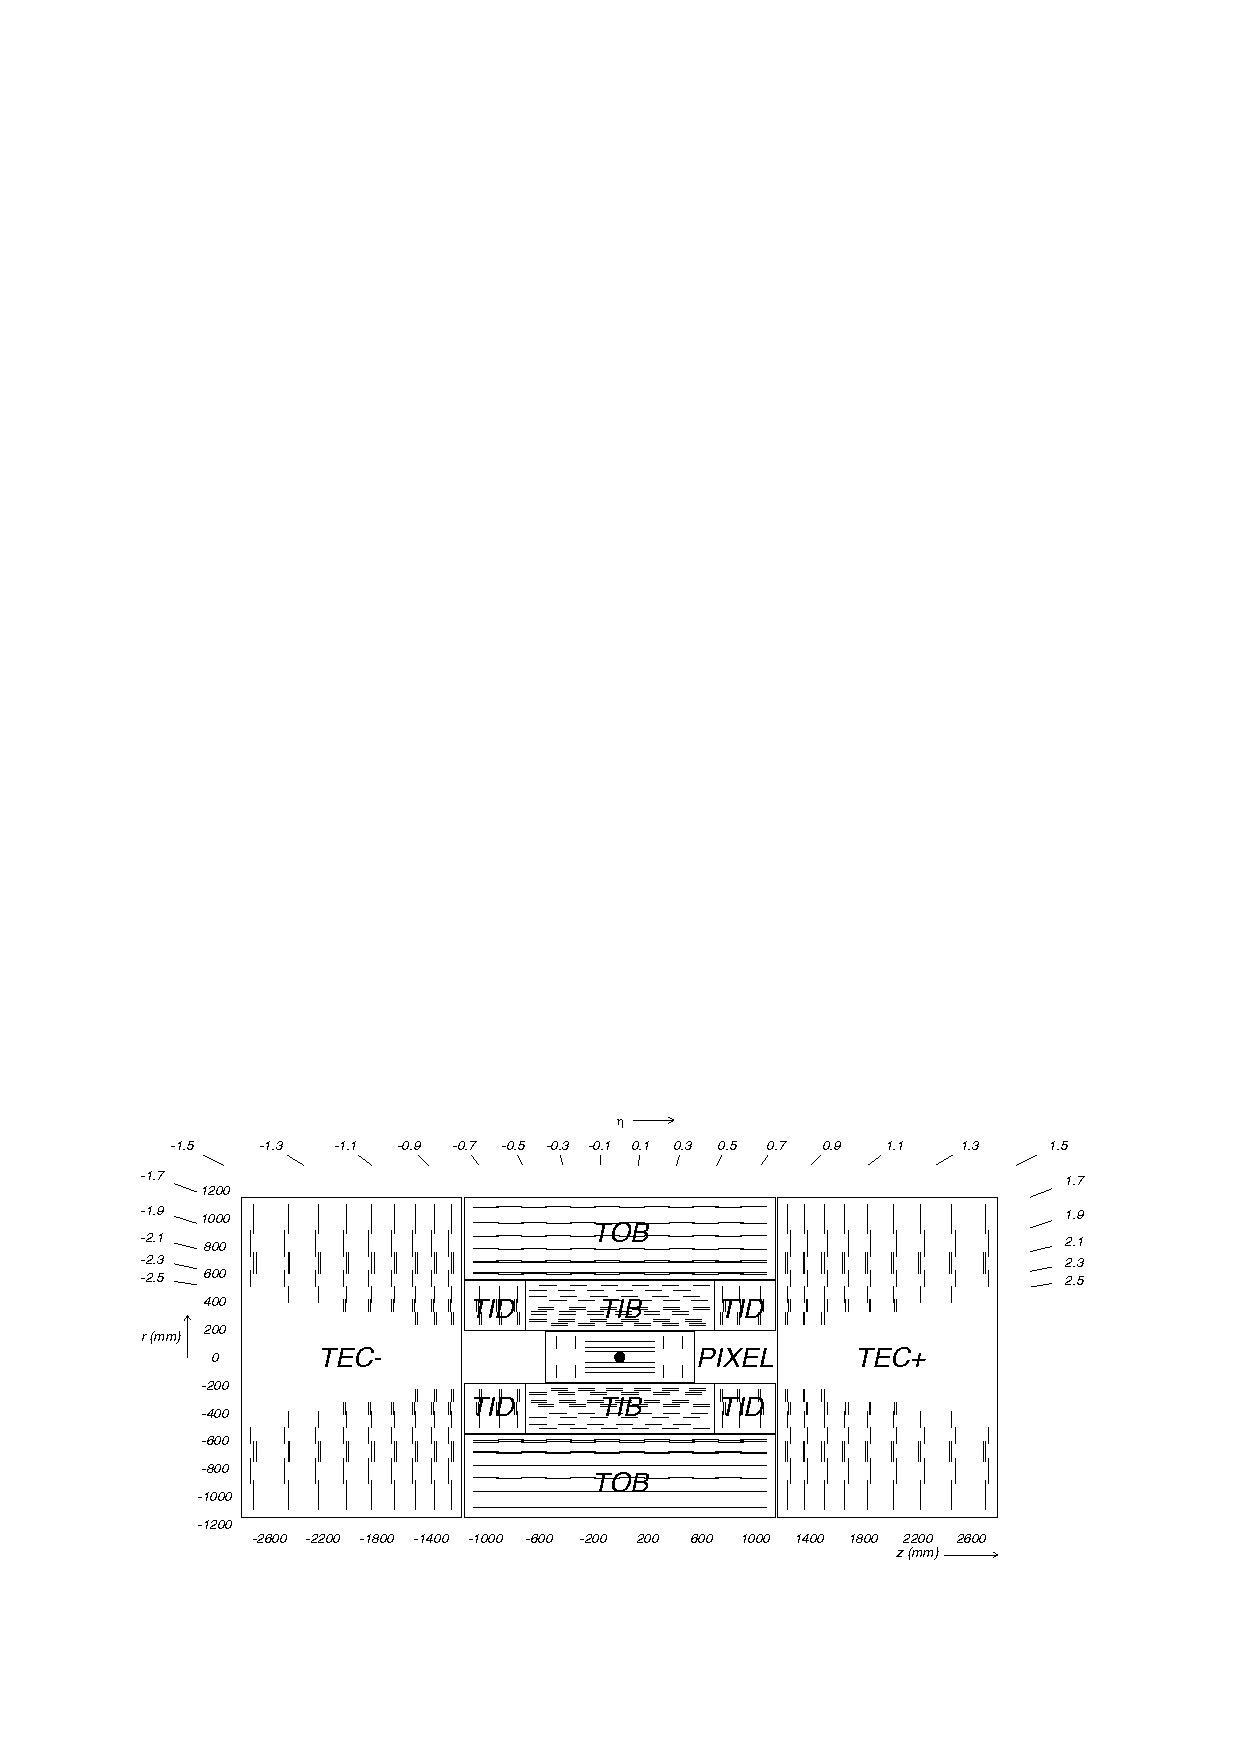
\includegraphics[width=0.8\textwidth]{fig/general_layout.pdf}
    \caption{Schematic cross section of the CMS Tracker.}
    \label{fig:tklayout}
  \end{center}
\end{figure}


The detection of photon conversions and nuclear interactions both rely
on the reconstruction of displaced secondary vertices, and the track
reconstruction algorithm described in~\cite{TRK-10-001} has been tuned
to allow reconstruction of tracks originated into the tracking volume,
as far as at a radius of $60\cm$.




{\bf lo usiamo questo che segue???}

The CMS tracker material is not negligible as a consequence of the
massive mechanical structure and the amount of services needed to
support and run such a large, complex and highly granular tracking device.

As a consequence of that, the effect of the interactions of particles
with the material are not negligible. 


A robust method for the Material Budget estimation, exploited by many
past experiments, is based on photon conversions. The idea is that the
material radiography, provided by the position of reconstructed photon
conversion vertices, allows for the visualisation of detector layers
and service structures and that the conversions rate, if properly
accounted, provides an estimate of the amount of material in the
detector volume.

At the LHC many photons are produced from $\pi^0$ decays in minimum bias events; 
as shown in Figure~\ref{ptMC}, the $p_T$ spectrum of such photons is
very soft and the electron and positron produced in the conversion 
do not have enough transverse momentum to reach the CMS electromagnetic calorimeter.
Therefore, conversions need to be reconstructed with a tracker standalone algorithm.

\begin{figure}[!hbtp]
\centering
%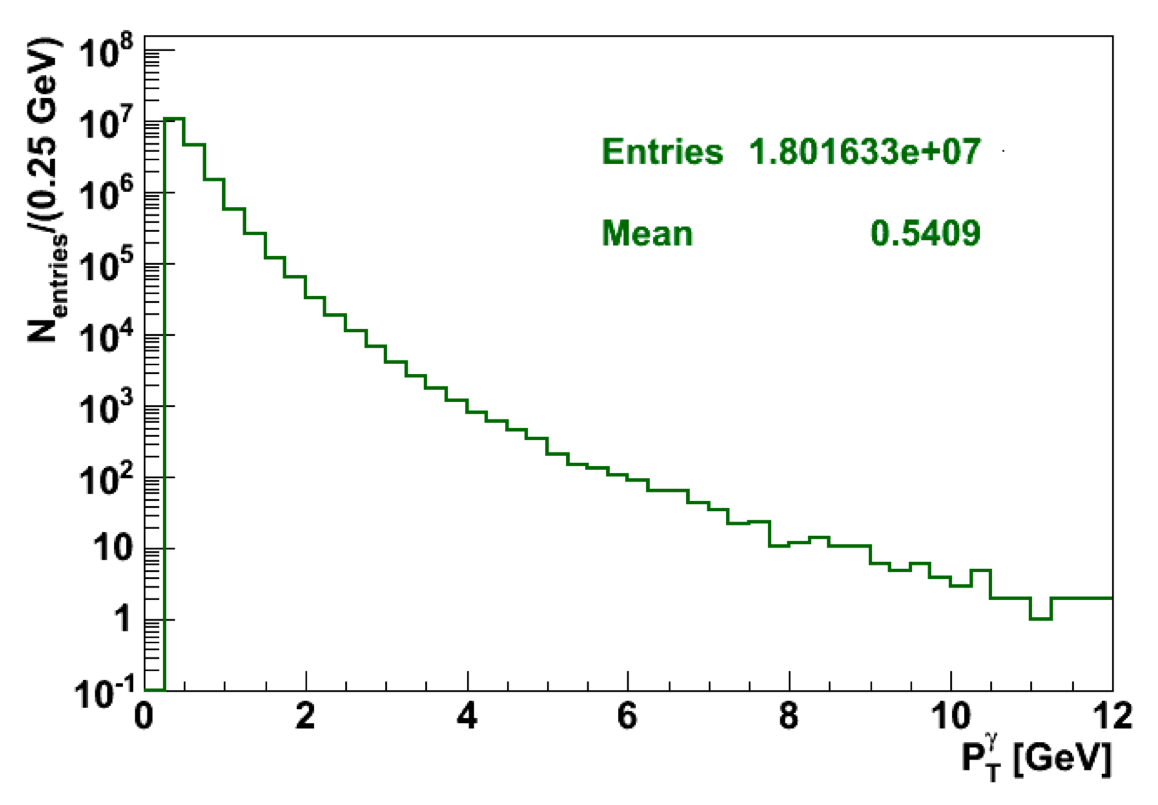
\includegraphics[width=.45\textwidth]{ptMC.png}
\caption{Transverse momentum spectrum of converted photons in minimum
  bias MC events at $\sqrt{s}=900\GeV$.}
\label{ptMC}
\end{figure}

The present analysis makes use of the algorithm described in~\cite{nancy}.
It allows the reconstruction of low-$p_T$ photons ($\geq 0.4\GeV$)
without any request of ECAL match. The main signature for the
conversion identification is the reconstruction of two opposite
charged tracks with tangent direction at the point where they form a
detached vertex. The vertex fit is performed with the \emph{Kinematic
  Constraint Vertex Fitter}.



